% This is a model template for the solutions in computational science. You can find a very useful documentation for LaTeX in Finnish at ftp://ftp.funet.fi/pub/TeX/CTAN/info/lshort/finnish/ or in English at ftp://ftp.funet.fi/pub/TeX/CTAN/info/lshort/english/. The section List of mathematical symbols in Chapter 3 is especially useful for the typesetting of mathematical formulas.

% Compile the document to PDF by command 'pdflatex model.tex' in the terminal. The command must be run twice for the references in the text to be correct.

\documentclass[a4paper,11pt]{article}
\usepackage[utf8]{inputenc}
% This includes letters such as � and �
\usepackage[T1]{fontenc}
% Use here 'Finnish' for Finnish hyphenation. You may have to compile the code twice after the change. 
\usepackage[english]{babel}
\usepackage{graphicx}
% Some math stuff
\usepackage{amsmath,amsfonts,amssymb,amsbsy,commath,booktabs,hyperref}  
% This is just to include the urls
\usepackage{hyperref,subcaption,verbatim}
\usepackage[margin=2cm]{geometry}

\setlength{\parindent}{0mm}
\setlength{\parskip}{1.0\baselineskip}
\usepackage{minted}
\usemintedstyle{tango}

\usepackage{listings}
\usepackage{color}
\usepackage{pdfpages}
\DeclareMathAlphabet{\pazocal}{OMS}{zplm}{m}{n}

\definecolor{dkgreen}{rgb}{0,0.6,0}
\definecolor{gray}{rgb}{0.5,0.5,0.5}
\definecolor{mauve}{rgb}{0.58,0,0.82}

\lstset{frame=tb,
	language=Python,
	aboveskip=3mm,
	belowskip=3mm,
	showstringspaces=false,
	columns=flexible,
	basicstyle={\tiny\ttfamily},
	numbers=none,
	numberstyle=\tiny\color{gray},
	keywordstyle=\color{blue},
	commentstyle=\color{dkgreen},
	stringstyle=\color{mauve},
	breaklines=true,
	breakatwhitespace=true,
	tabsize=4
}

\begin{document}

\title{CS-E4830 Kernel Methods in Machine Learning \\ Assignment 3} % Replace the exercise round number
\author{Kunal Ghosh, 546247} % Replace with your name and student number
\maketitle
\section*{}
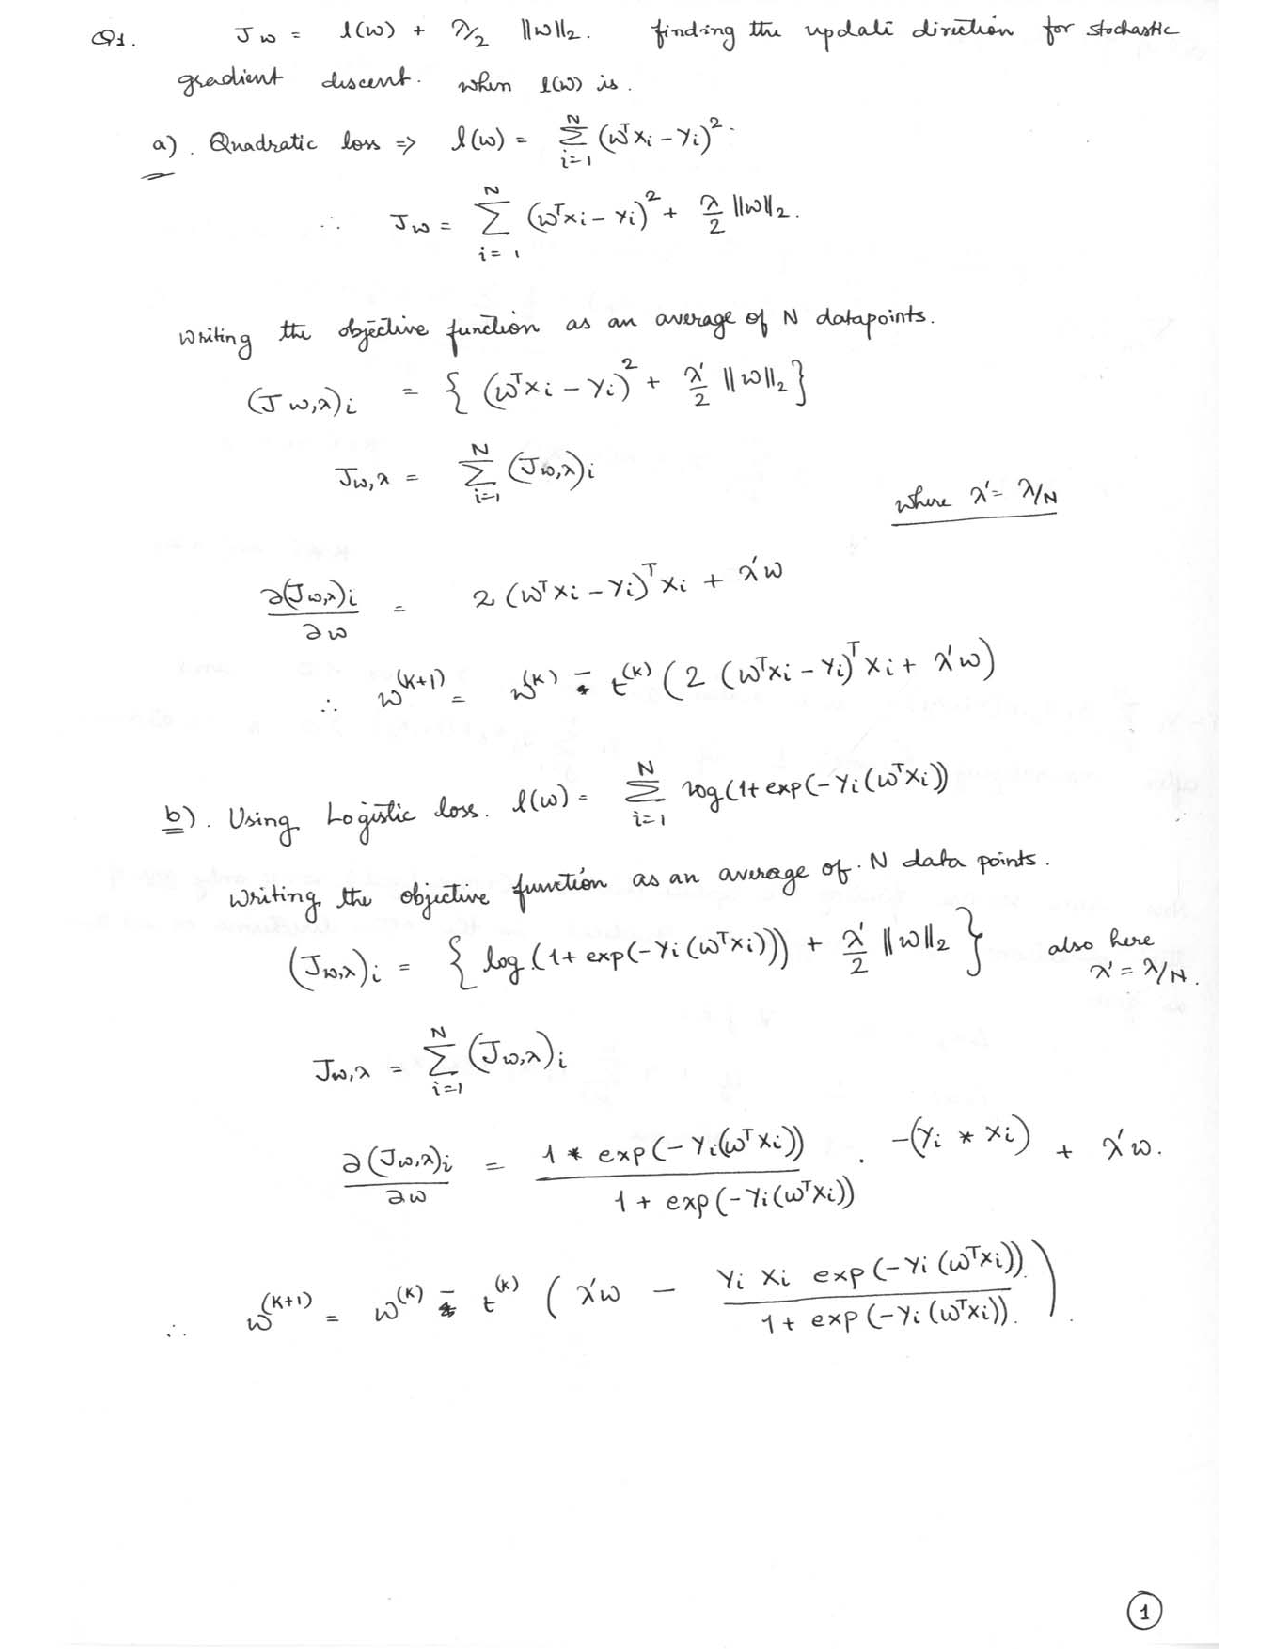
\includepdf[pages=-]{assignment3q1n2-1.pdf}
\section*{Solution to Question 3(a)}
Implementation of the \texttt{Stochastic Dual Coordinate Ascent for SVM} as described in the Assignment handout.
\inputminted[baselinestretch=1, fontsize=\small, breaklines=true, mathescape]{python}{../svmTrainDCGA2.py}
\section*{Solution to Question 3(b)}
In this section we have used the Quadratic program solver of the \texttt{CVXOPT} package in python, to solve
dual soft-margin SVM (equation 1 as given in the assignment handout).
\inputminted[baselinestretch=1, fontsize=\small, breaklines=true, mathescape]{python}{../svmTrainQP.py}
\section*{Solution to Question 3(c)}
We have used the following code snippet to run the \texttt{svmTrainDCGA} and \texttt{svmTrainQP} for different amounts
of training data. It also contains the code to time the execution, calculate prediction accuracy and generate plots.  
The plot thus generated are discussed in the next section.
\inputminted[baselinestretch=1, fontsize=\small, breaklines=true, mathescape]{python}{../Assignment3.py}

\section*{Solution to Question 3(d)}
\begin{figure}[ht]
    \centering
    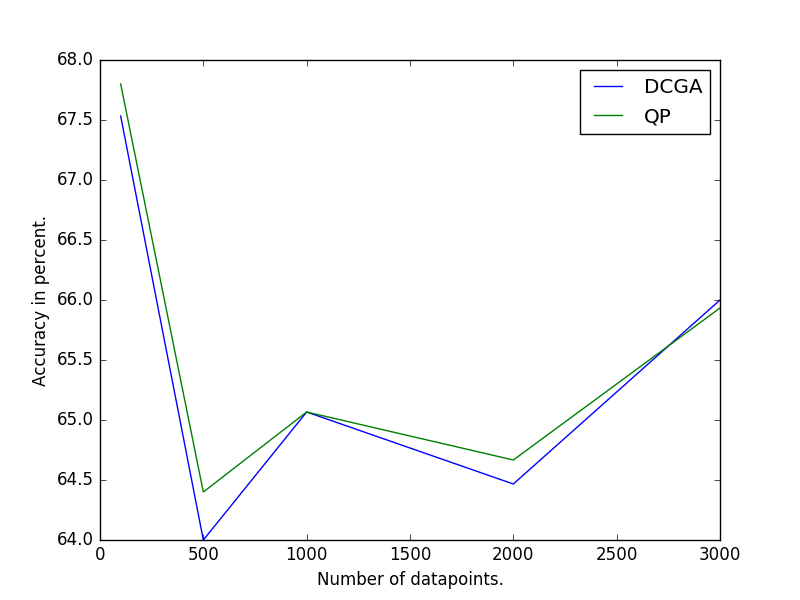
\includegraphics[width=1.1\linewidth]{figure_11.png}
    \label{fig:f11}
    \caption{\textit{This figure shows the test accuracy in percentage as a function of the training dataset size. It can be seen that the \texttt{Stochastic Dual Coordinate Ascent (DCGA)}
    algorithm performs better than the \texttt{Quadratic Program} solver for the full dataset but has lower accuracy for small dataset size. \textbf{Note!} that the same trend wasn't visible over multiple runs (see Figure 2 for another run). However, for the full dataset Stochastic DCGA did perform better than the QP version consistently. 
    }}
\end{figure}
\begin{figure}[ht]
    \centering
    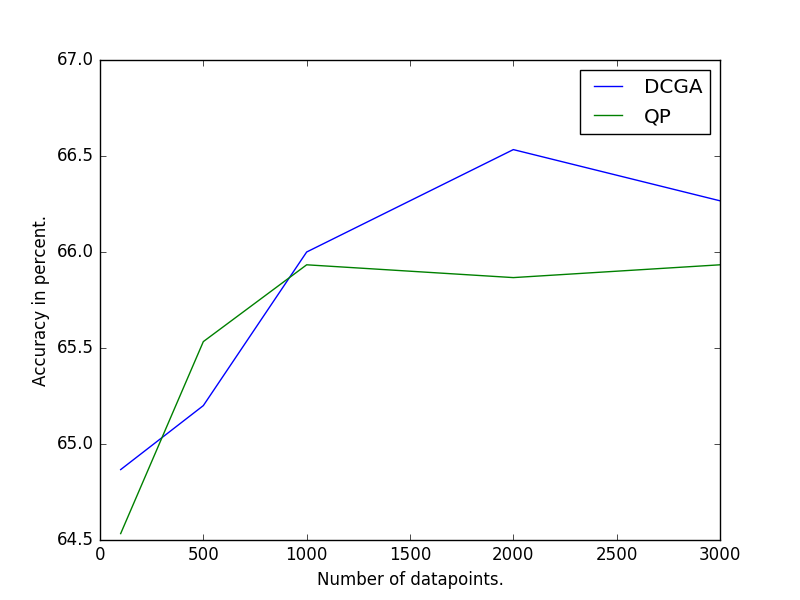
\includegraphics[width=1.1\linewidth]{figure_12.png}
    \label{fig:f12}
    \caption{\textit{This figure shows the test accuracy in percentage as a function of the training dataset size. This is an alternate run of the same code used to generate Figure 1, it is clear that \texttt{Stochastic DCGA} performs bettern than the \texttt{QP} for a given fixed dataset (all 3000 datapoints) but one cannot make the same conclusion for smaller dataset sizes as there is quite a lot of variance in the accuracy as is seen by comparing this figure with Figure 1.}} 
\end{figure}

\begin{figure}[ht]
    \centering
    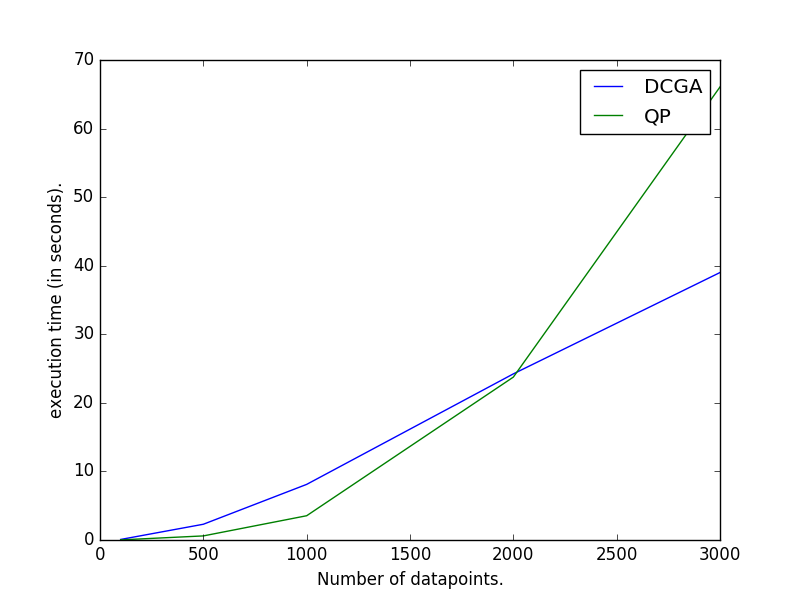
\includegraphics[width=1.1\linewidth]{runtime.png}
    \label{fig:f2}
    \caption{\textit{This figure shows the execution time (seconds), lower is better, as a function of the number of training datapoints. It is quite clear that the Quadratic programming \texttt{(QP)} solution is faster for small to moderate dataset sizes as compared to the \texttt{Stochastic DCGA} implementation. However as the dataset size increases \texttt{Stochastic DCGA} starts to run much quicker than the \texttt{QP}.}}
\end{figure}


\end{document}

   

